\documentclass[11pt,letterpaper]{article}
\usepackage[margin=.65in,headheight=16pt,headsep=.15in,footskip=.3in]{geometry}
\usepackage[T1]{fontenc}
\usepackage[default]{sourcesanspro}
\usepackage{tikz,fancyhdr}
\usetikzlibrary{arrows.meta,calc,decorations.markings}
\setlength{\parindent}{0pt}
\setlength{\parskip}{.08in}
\pagestyle{fancy}\fancyhf{}
\renewcommand{\headrulewidth}{.4pt}
\renewcommand{\footrulewidth}{.4pt}
\fancyfoot[L]{\small Bellingham Math Circle / Week 10 / F10-RV-v1}
\fancyfoot[R]{\small\thepage}
\newcommand{\band}[2]{\fancyhead[L]{Week 10 / #1 / Grades #2}}
\newcommand{\problem}[2]{\par\textbf{Problem #1:} #2\par}
\newcommand{\continued}[2]{\par Problem #1 continued. #2\par}
\tikzset{
 street/.style={line width=1.2pt},
 arrowstreet/.style={postaction={decorate},decoration={markings,mark=at position .86 with {\arrow{Stealth[length=3mm,width=2.4mm]}}}},
 demoarrow/.style={postaction={decorate},decoration={markings,mark=at position .72 with {\arrow{Stealth[length=2mm,width=1.6mm]}}}},
 island/.style={circle,draw,line width=.8pt,fill=white,minimum size=.3in,inner sep=0,font=\normalsize},
 counter/.style={circle,draw,fill=white,line width=.8pt,minimum size=.14in,inner sep=0},
 demostreet/.style={line width=.8pt},
 demoused/.style={draw=gray!60,line width=.8pt,dashed},
 democounter/.style={circle,draw,fill=white,line width=.7pt,minimum size=.08in,inner sep=0},
 demoisland/.style={circle,draw,fill=white,minimum size=.2in,inner sep=0,font=\scriptsize}
}
\begin{document}

\band{Arrow streets}{K--5}
Follow the arrows. Pick up each street's counter as you cross. The ring shows the walker. Put all counters back before another try.
\begin{center}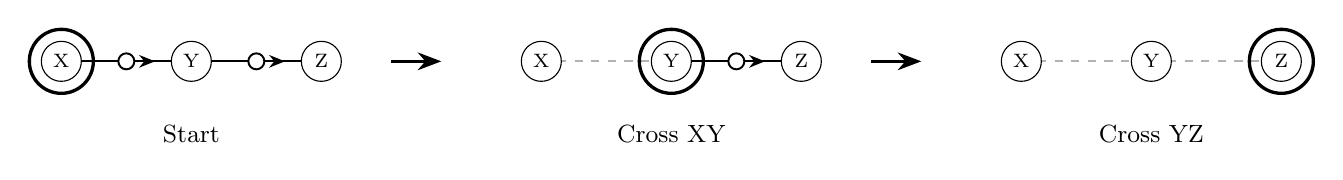
\begin{tikzpicture}[x=1in,y=1in]
\begin{scope}[shift={(0.0,0)}]
\coordinate (X) at (0.15,0.4);
\coordinate (Y) at (0.8,0.4);
\coordinate (Z) at (1.45,0.4);
\draw[demostreet,demoarrow] (X) -- (Y);
\node[democounter] at ($(X)!.5!(Y)$) {};
\draw[demostreet,demoarrow] (Y) -- (Z);
\node[democounter] at ($(Y)!.5!(Z)$) {};
\node[demoisland] at (X) {X};
\node[demoisland] at (Y) {Y};
\node[demoisland] at (Z) {Z};
\draw[line width=1.2pt] (X) circle (.16);
\node[anchor=north,font=\small] at (.8,.13) {Start};
\end{scope}
\draw[-{Stealth[length=3mm]},line width=1pt] (1.8,.4)--(2.05,.4);
\begin{scope}[shift={(2.4,0)}]
\coordinate (X) at (0.15,0.4);
\coordinate (Y) at (0.8,0.4);
\coordinate (Z) at (1.45,0.4);
\draw[demoused] (X) -- (Y);
\draw[demostreet,demoarrow] (Y) -- (Z);
\node[democounter] at ($(Y)!.5!(Z)$) {};
\node[demoisland] at (X) {X};
\node[demoisland] at (Y) {Y};
\node[demoisland] at (Z) {Z};
\draw[line width=1.2pt] (Y) circle (.16);
\node[anchor=north,font=\small] at (.8,.13) {Cross XY};
\end{scope}
\draw[-{Stealth[length=3mm]},line width=1pt] (4.2,.4)--(4.449999999999999,.4);
\begin{scope}[shift={(4.8,0)}]
\coordinate (X) at (0.15,0.4);
\coordinate (Y) at (0.8,0.4);
\coordinate (Z) at (1.45,0.4);
\draw[demoused] (X) -- (Y);
\draw[demoused] (Y) -- (Z);
\node[demoisland] at (X) {X};
\node[demoisland] at (Y) {Y};
\node[demoisland] at (Z) {Z};
\draw[line width=1.2pt] (Z) circle (.16);
\node[anchor=north,font=\small] at (.8,.13) {Cross YZ};
\end{scope}
\end{tikzpicture}\end{center}
\problem{1}{Which towns can you walk through using every street exactly once? Start wherever you choose.}
\noindent\begin{minipage}{.49\linewidth}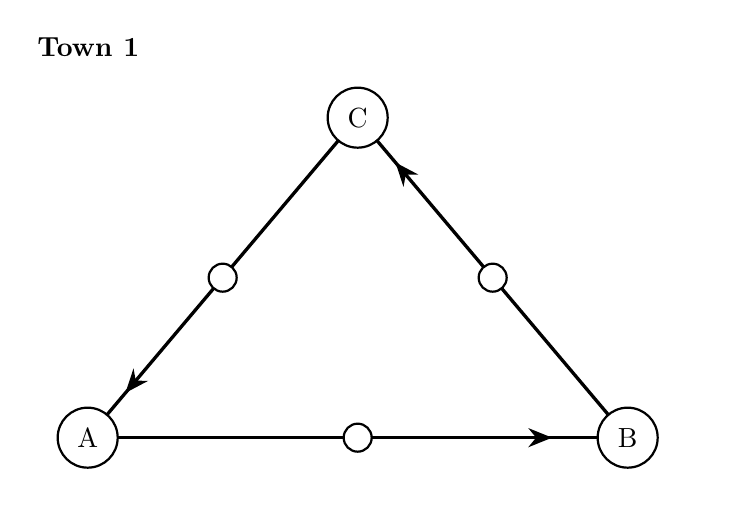
\begin{tikzpicture}[x=1in,y=1in]
\path[use as bounding box] (0,0) rectangle (3.4,2.35);
\node[anchor=north west,font=\bfseries] at (0,2.35) {Town 1};
\coordinate (A) at (0.3,0.3);
\coordinate (B) at (3.0,0.3);
\coordinate (C) at (1.65,1.9);
\draw[street,arrowstreet] (A) -- (B);
\node[counter] at ($(A)!.5!(B)$) {};
\draw[street,arrowstreet] (B) -- (C);
\node[counter] at ($(B)!.5!(C)$) {};
\draw[street,arrowstreet] (C) -- (A);
\node[counter] at ($(C)!.5!(A)$) {};
\node[island] at (A) {A};
\node[island] at (B) {B};
\node[island] at (C) {C};
\end{tikzpicture}\end{minipage}\hfill\begin{minipage}{.49\linewidth}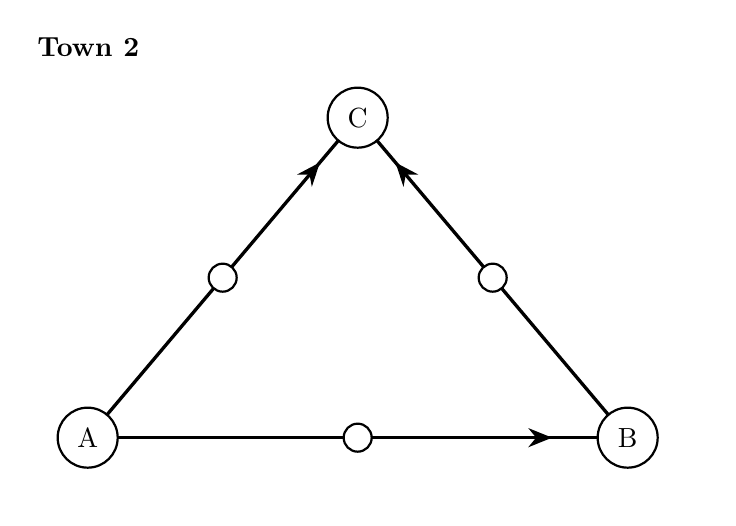
\begin{tikzpicture}[x=1in,y=1in]
\path[use as bounding box] (0,0) rectangle (3.4,2.35);
\node[anchor=north west,font=\bfseries] at (0,2.35) {Town 2};
\coordinate (A) at (0.3,0.3);
\coordinate (B) at (3.0,0.3);
\coordinate (C) at (1.65,1.9);
\draw[street,arrowstreet] (A) -- (B);
\node[counter] at ($(A)!.5!(B)$) {};
\draw[street,arrowstreet] (A) -- (C);
\node[counter] at ($(A)!.5!(C)$) {};
\draw[street,arrowstreet] (B) -- (C);
\node[counter] at ($(B)!.5!(C)$) {};
\node[island] at (A) {A};
\node[island] at (B) {B};
\node[island] at (C) {C};
\end{tikzpicture}\end{minipage}\par\vspace{.13in}
\noindent\begin{minipage}{.49\linewidth}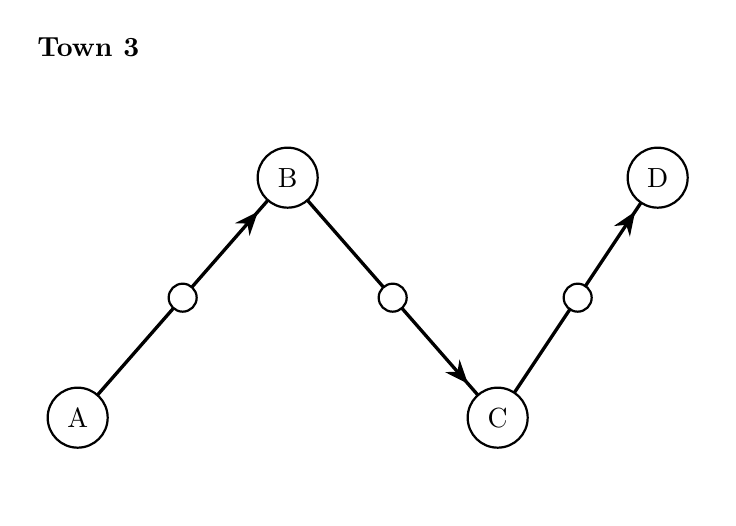
\begin{tikzpicture}[x=1in,y=1in]
\path[use as bounding box] (0,0) rectangle (3.4,2.35);
\node[anchor=north west,font=\bfseries] at (0,2.35) {Town 3};
\coordinate (A) at (0.25,0.4);
\coordinate (B) at (1.3,1.6);
\coordinate (C) at (2.35,0.4);
\coordinate (D) at (3.15,1.6);
\draw[street,arrowstreet] (A) -- (B);
\node[counter] at ($(A)!.5!(B)$) {};
\draw[street,arrowstreet] (B) -- (C);
\node[counter] at ($(B)!.5!(C)$) {};
\draw[street,arrowstreet] (C) -- (D);
\node[counter] at ($(C)!.5!(D)$) {};
\node[island] at (A) {A};
\node[island] at (B) {B};
\node[island] at (C) {C};
\node[island] at (D) {D};
\end{tikzpicture}\end{minipage}\hfill\begin{minipage}{.49\linewidth}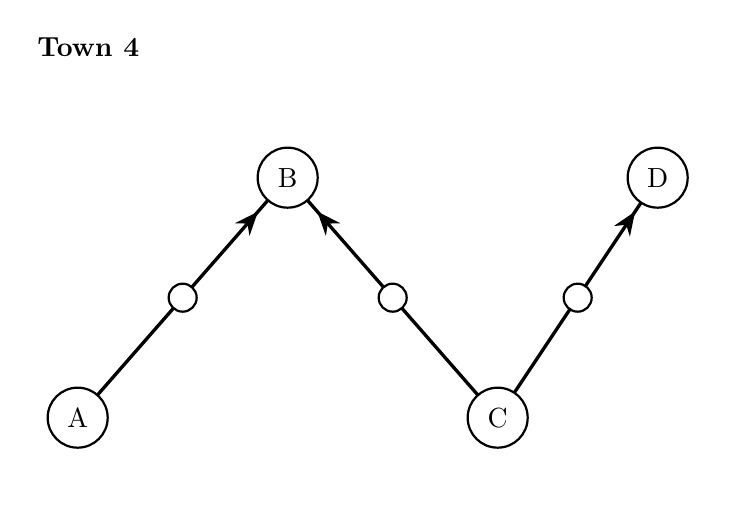
\begin{tikzpicture}[x=1in,y=1in]
\path[use as bounding box] (0,0) rectangle (3.4,2.35);
\node[anchor=north west,font=\bfseries] at (0,2.35) {Town 4};
\coordinate (A) at (0.25,0.4);
\coordinate (B) at (1.3,1.6);
\coordinate (C) at (2.35,0.4);
\coordinate (D) at (3.15,1.6);
\draw[street,arrowstreet] (A) -- (B);
\node[counter] at ($(A)!.5!(B)$) {};
\draw[street,arrowstreet] (C) -- (B);
\node[counter] at ($(C)!.5!(B)$) {};
\draw[street,arrowstreet] (C) -- (D);
\node[counter] at ($(C)!.5!(D)$) {};
\node[island] at (A) {A};
\node[island] at (B) {B};
\node[island] at (C) {C};
\node[island] at (D) {D};
\end{tikzpicture}\end{minipage}\par\vspace{.13in}
\newpage\band{Arrow streets}{2--5}
\continued{1}{Which towns can you walk through using every street exactly once? Start wherever you choose.}
\begin{center}\begin{tikzpicture}[x=1in,y=1in]
\path[use as bounding box] (0,0) rectangle (6.8,3.2);
\node[anchor=north west,font=\bfseries] at (0,3.2) {Town 5};
\coordinate (A) at (1.0,0.3);
\coordinate (B) at (5.5,0.3);
\coordinate (C) at (5.5,2.5);
\coordinate (D) at (1.0,2.5);
\draw[street,arrowstreet] (A) -- (B);
\node[counter] at ($(A)!.5!(B)$) {};
\draw[street,arrowstreet] (B) -- (C);
\node[counter] at ($(B)!.5!(C)$) {};
\draw[street,arrowstreet] (C) -- (D);
\node[counter] at ($(C)!.5!(D)$) {};
\draw[street,arrowstreet] (D) -- (A);
\node[counter] at ($(D)!.5!(A)$) {};
\draw[street,arrowstreet] (A) -- (C);
\node[counter] at ($(A)!.5!(C)$) {};
\node[island] at (A) {A};
\node[island] at (B) {B};
\node[island] at (C) {C};
\node[island] at (D) {D};
\end{tikzpicture}\end{center}
\vspace{.15in}
\begin{center}\begin{tikzpicture}[x=1in,y=1in]
\path[use as bounding box] (0,0) rectangle (6.8,3.2);
\node[anchor=north west,font=\bfseries] at (0,3.2) {Town 6};
\coordinate (A) at (1.0,0.3);
\coordinate (B) at (5.5,0.3);
\coordinate (C) at (5.5,2.5);
\coordinate (D) at (1.0,2.5);
\draw[street,arrowstreet] (A) -- (B);
\node[counter] at ($(A)!.5!(B)$) {};
\draw[street,arrowstreet] (B) -- (C);
\node[counter] at ($(B)!.5!(C)$) {};
\draw[street,arrowstreet] (D) -- (C);
\node[counter] at ($(D)!.5!(C)$) {};
\draw[street,arrowstreet] (D) -- (A);
\node[counter] at ($(D)!.5!(A)$) {};
\draw[street,arrowstreet] (A) -- (C);
\node[counter] at ($(A)!.5!(C)$) {};
\node[island] at (A) {A};
\node[island] at (B) {B};
\node[island] at (C) {C};
\node[island] at (D) {D};
\end{tikzpicture}\end{center}
\vspace{.15in}
\newpage\band{Arrow streets}{2--5}
\continued{1}{Which towns can you walk through using every street exactly once? Start wherever you choose.}
\begin{center}\begin{tikzpicture}[x=1in,y=1in]
\path[use as bounding box] (0,0) rectangle (6.8,3.2);
\node[anchor=north west,font=\bfseries] at (0,3.2) {Town 7};
\coordinate (A) at (0.45,0.3);
\coordinate (B) at (2.85,0.3);
\coordinate (C) at (1.65,2.5);
\coordinate (D) at (3.95,0.3);
\coordinate (E) at (6.35,0.3);
\coordinate (F) at (5.15,2.5);
\draw[street,arrowstreet] (A) -- (B);
\node[counter] at ($(A)!.5!(B)$) {};
\draw[street,arrowstreet] (B) -- (C);
\node[counter] at ($(B)!.5!(C)$) {};
\draw[street,arrowstreet] (C) -- (A);
\node[counter] at ($(C)!.5!(A)$) {};
\draw[street,arrowstreet] (D) -- (E);
\node[counter] at ($(D)!.5!(E)$) {};
\draw[street,arrowstreet] (E) -- (F);
\node[counter] at ($(E)!.5!(F)$) {};
\draw[street,arrowstreet] (F) -- (D);
\node[counter] at ($(F)!.5!(D)$) {};
\node[island] at (A) {A};
\node[island] at (B) {B};
\node[island] at (C) {C};
\node[island] at (D) {D};
\node[island] at (E) {E};
\node[island] at (F) {F};
\end{tikzpicture}\end{center}
\vspace{.15in}
\begin{center}\begin{tikzpicture}[x=1in,y=1in]
\path[use as bounding box] (0,0) rectangle (6.8,3.2);
\node[anchor=north west,font=\bfseries] at (0,3.2) {Town 8};
\coordinate (A) at (3.4,1.4);
\coordinate (B) at (0.45,0.3);
\coordinate (C) at (0.45,2.5);
\coordinate (D) at (6.35,2.5);
\coordinate (E) at (6.35,0.3);
\draw[street,arrowstreet] (A) -- (B);
\node[counter] at ($(A)!.5!(B)$) {};
\draw[street,arrowstreet] (B) -- (C);
\node[counter] at ($(B)!.5!(C)$) {};
\draw[street,arrowstreet] (C) -- (A);
\node[counter] at ($(C)!.5!(A)$) {};
\draw[street,arrowstreet] (A) -- (D);
\node[counter] at ($(A)!.5!(D)$) {};
\draw[street,arrowstreet] (D) -- (E);
\node[counter] at ($(D)!.5!(E)$) {};
\draw[street,arrowstreet] (E) -- (A);
\node[counter] at ($(E)!.5!(A)$) {};
\node[island] at (A) {A};
\node[island] at (B) {B};
\node[island] at (C) {C};
\node[island] at (D) {D};
\node[island] at (E) {E};
\end{tikzpicture}\end{center}
\vspace{.15in}
\newpage\band{Route choices}{2--5}
Streets may be crossed either way. Pick up each street's counter as you cross. Start at the star. Before another try, put all counters back and return to the star.
\problem{2}{Which streets can you cross first and still use every street exactly once? Mark those streets.}
\begin{center}\begin{tikzpicture}[x=1in,y=1in]
\path[use as bounding box] (0,0) rectangle (6.8,3.2);
\node[anchor=north west,font=\bfseries] at (0,3.2) {Town 1};
\coordinate (A) at (3.2,1.5);
\coordinate (B) at (0.6,0.3);
\coordinate (C) at (0.6,2.65);
\coordinate (D) at (6.3,1.5);
\draw[street] (A) -- (B);
\node[counter] at ($(A)!.5!(B)$) {};
\draw[street] (B) -- (C);
\node[counter] at ($(B)!.5!(C)$) {};
\draw[street] (C) -- (A);
\node[counter] at ($(C)!.5!(A)$) {};
\draw[street] (A) -- (D);
\node[counter] at ($(A)!.5!(D)$) {};
\node[island] at (A) {A};
\node[island] at (B) {B};
\node[island] at (C) {C};
\node[island] at (D) {D};
\node[font=\Large,anchor=south] at ($(A)+(0,.18)$) {$\star$};
\end{tikzpicture}\end{center}
\vspace{.15in}
\begin{center}\begin{tikzpicture}[x=1in,y=1in]
\path[use as bounding box] (0,0) rectangle (6.8,3.2);
\node[anchor=north west,font=\bfseries] at (0,3.2) {Town 2};
\coordinate (A) at (3.2,1.5);
\coordinate (B) at (0.6,0.3);
\coordinate (C) at (0.6,2.65);
\coordinate (D) at (6.3,1.5);
\draw[street] (A) -- (B);
\node[counter] at ($(A)!.5!(B)$) {};
\draw[street] (B) -- (C);
\node[counter] at ($(B)!.5!(C)$) {};
\draw[street] (C) -- (A);
\node[counter] at ($(C)!.5!(A)$) {};
\draw[street] (A) -- (D);
\node[counter] at ($(A)!.5!(D)$) {};
\node[island] at (A) {A};
\node[island] at (B) {B};
\node[island] at (C) {C};
\node[island] at (D) {D};
\node[font=\Large,anchor=south] at ($(D)+(0,.18)$) {$\star$};
\end{tikzpicture}\end{center}
\vspace{.15in}
\newpage\band{Route choices}{2--5}
\continued{2}{Which streets can you cross first and still use every street exactly once? Mark those streets.}
\begin{center}\begin{tikzpicture}[x=1in,y=1in]
\path[use as bounding box] (0,0) rectangle (6.8,3.2);
\node[anchor=north west,font=\bfseries] at (0,3.2) {Town 3};
\coordinate (A) at (1.0,0.3);
\coordinate (B) at (5.5,0.3);
\coordinate (C) at (5.5,2.5);
\coordinate (D) at (1.0,2.5);
\draw[street] (A) -- (B);
\node[counter] at ($(A)!.5!(B)$) {};
\draw[street] (B) -- (C);
\node[counter] at ($(B)!.5!(C)$) {};
\draw[street] (C) -- (D);
\node[counter] at ($(C)!.5!(D)$) {};
\draw[street] (D) -- (A);
\node[counter] at ($(D)!.5!(A)$) {};
\draw[street] (A) -- (C);
\node[counter] at ($(A)!.5!(C)$) {};
\node[island] at (A) {A};
\node[island] at (B) {B};
\node[island] at (C) {C};
\node[island] at (D) {D};
\node[font=\Large,anchor=east] at ($(A)+(-.18,0)$) {$\star$};
\end{tikzpicture}\end{center}
\vspace{.15in}
\begin{center}\begin{tikzpicture}[x=1in,y=1in]
\path[use as bounding box] (0,0) rectangle (6.8,3.2);
\node[anchor=north west,font=\bfseries] at (0,3.2) {Town 4};
\coordinate (A) at (2.5,1.5);
\coordinate (B) at (0.35,0.3);
\coordinate (C) at (0.35,2.7);
\coordinate (D) at (4.3,1.5);
\coordinate (E) at (6.45,0.3);
\coordinate (F) at (6.45,2.7);
\draw[street] (A) -- (B);
\node[counter] at ($(A)!.5!(B)$) {};
\draw[street] (B) -- (C);
\node[counter] at ($(B)!.5!(C)$) {};
\draw[street] (C) -- (A);
\node[counter] at ($(C)!.5!(A)$) {};
\draw[street] (A) -- (D);
\node[counter] at ($(A)!.5!(D)$) {};
\draw[street] (D) -- (E);
\node[counter] at ($(D)!.5!(E)$) {};
\draw[street] (E) -- (F);
\node[counter] at ($(E)!.5!(F)$) {};
\draw[street] (F) -- (D);
\node[counter] at ($(F)!.5!(D)$) {};
\node[island] at (A) {A};
\node[island] at (B) {B};
\node[island] at (C) {C};
\node[island] at (D) {D};
\node[island] at (E) {E};
\node[island] at (F) {F};
\node[font=\Large,anchor=south] at ($(A)+(0,.18)$) {$\star$};
\end{tikzpicture}\end{center}
\vspace{.15in}
\newpage\band{Password windows}{4--5}
A window reads neighboring buttons from left to right. In this two-button example, the window slides one place each time.
\begin{center}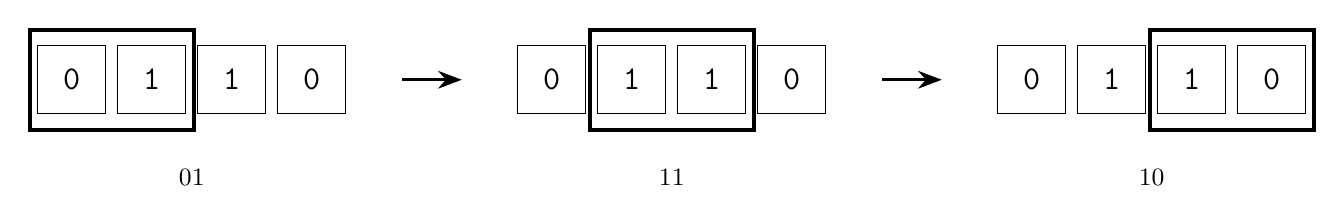
\begin{tikzpicture}[x=1in,y=1in]
\foreach \k in {0,1,2} {
  \begin{scope}[shift={(2.4*\k,0)}]
    \foreach \d [count=\j from 0] in {0,1,1,0}
      \node[draw,minimum size=.34in,inner sep=0,font=\large\ttfamily] at (.4*\j,.8) {\d};
    \draw[line width=1.5pt] (.4*\k-.21,.55) rectangle (.4*\k+.61,1.05);
    \node[anchor=north,font=\small] at (.6,.4) {\ifcase\k\relax 01\or 11\or 10\fi};
  \end{scope}
}
\draw[-{Stealth[length=3mm]},line width=1pt] (1.65,.8)--(1.95,.8);
\draw[-{Stealth[length=3mm]},line width=1pt] (4.05,.8)--(4.35,.8);
\end{tikzpicture}\end{center}
\problem{3}{Make a row of 0 and 1 tiles containing all eight three-button passwords below. How few tiles can you use?}

\begin{center}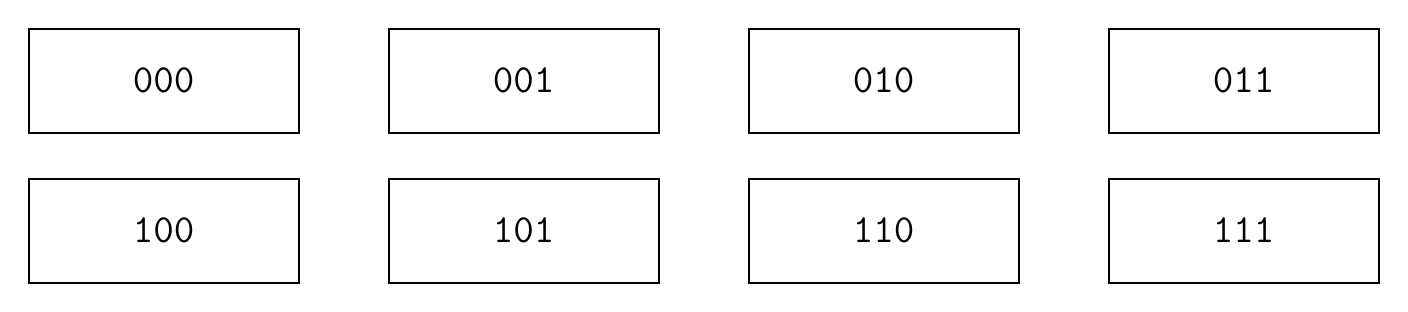
\begin{tikzpicture}[x=1in,y=1in]
\foreach \s [count=\i from 0] in {000,001,010,011,100,101,110,111} {
  \pgfmathtruncatemacro{\col}{mod(\i,4)}
  \pgfmathtruncatemacro{\row}{int(\i/4)}
  \node[draw,line width=.7pt,minimum width=1.35in,minimum height=.52in,font=\Large\ttfamily]
    at (1.8*\col,-.75*\row) {\s};
}
\end{tikzpicture}\end{center}

\vspace{.25in}
\begin{tikzpicture}[x=1in,y=1in]
\foreach \y in {0,1.35,2.7} \draw[gray!45,dashed] (0,\y) rectangle (7.1,\y+1.05);
\end{tikzpicture}

\newpage\band{Password windows}{4--5}
Read a circle clockwise. A window may cross the join. This two-button circle has three windows.
\begin{center}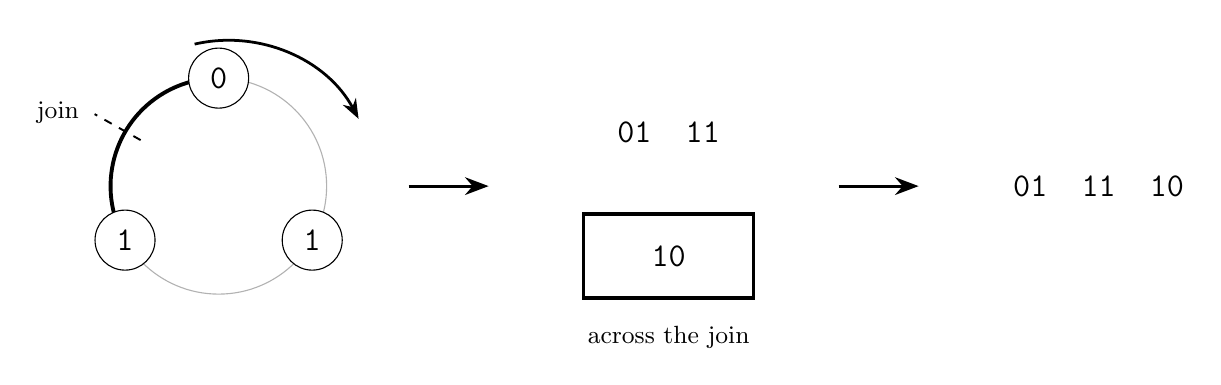
\begin{tikzpicture}[x=1in,y=1in]
\draw[gray!60] (.65,.85) circle (.54);
\draw[line width=1.4pt] (.182,.58) arc[start angle=210,end angle=90,radius=.54];
\draw[dashed,line width=.7pt] (.26,1.08)--(.03,1.21);
\node[anchor=east,font=\small] at (0,1.22) {join};
\node[draw,circle,fill=white,minimum size=.3in,inner sep=0,font=\large\ttfamily] (c0) at (.65,1.39) {0};
\node[draw,circle,fill=white,minimum size=.3in,inner sep=0,font=\large\ttfamily] (c1) at (1.118,.58) {1};
\node[draw,circle,fill=white,minimum size=.3in,inner sep=0,font=\large\ttfamily] (c2) at (.182,.58) {1};
\draw[-{Stealth[length=2.5mm]},line width=1pt] (.53,1.56) arc[start angle=103,end angle=28,radius=.74];
\draw[-{Stealth[length=3mm]},line width=1pt] (1.6,.85)--(2.0,.85);
\node[anchor=center,font=\large\ttfamily] at (2.9,1.12) {01\quad11};
\node[draw,line width=1.3pt,minimum width=.85in,minimum height=.42in,font=\large\ttfamily] at (2.9,.5) {10};
\node[anchor=north,font=\small] at (2.9,.2) {across the join};
\draw[-{Stealth[length=3mm]},line width=1pt] (3.75,.85)--(4.15,.85);
\node[font=\large\ttfamily,align=left] at (5.05,.85) {01\quad11\quad10};
\end{tikzpicture}\end{center}
\continued{3}{Make a circle of 0 and 1 tiles containing all eight three-button passwords. What is the fewest tiles you can use?}

\begin{center}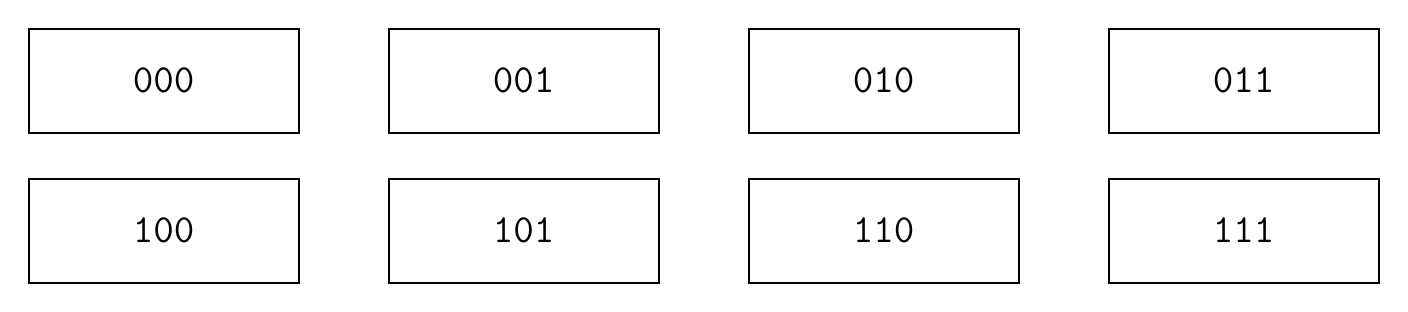
\begin{tikzpicture}[x=1in,y=1in]
\foreach \s [count=\i from 0] in {000,001,010,011,100,101,110,111} {
  \pgfmathtruncatemacro{\col}{mod(\i,4)}
  \pgfmathtruncatemacro{\row}{int(\i/4)}
  \node[draw,line width=.7pt,minimum width=1.35in,minimum height=.52in,font=\Large\ttfamily]
    at (1.8*\col,-.75*\row) {\s};
}
\end{tikzpicture}\end{center}

\vspace{.2in}
\begin{center}\begin{tikzpicture}[x=1in,y=1in]
\draw[gray!45,dashed] (1.65,1.7) circle (1.55);
\draw[gray!45,dashed] (5.4,1.7) circle (1.55);
\end{tikzpicture}\end{center}
\end{document}
